\documentclass[a4paper, 11pt, titlepage]{article}
% \usepackage{geometry}
% \usepackage{longtable}
\usepackage{tabularx}
\usepackage{setspace}
\usepackage[backend=biber]{biblatex}
\usepackage{bm}
\usepackage{amsmath}
\usepackage{hyperref}
\usepackage{graphicx,float}
\usepackage[export]{adjustbox}
\usepackage{listings}
\lstset{
basicstyle=\small\ttfamily,
columns=flexible,
breaklines=true
}

% \nocite{*}

\title{COMP5900C\\
Assignment 2\\
Non-Parametric Texture Synthesis}
\author{Gabriel Racz}
\date{March 2, 2025}

\begin{document}
\maketitle
\section{Implementation}
\subsection{Pixel-based}
My pixel-based method is designed with flexibility and simplicity in mind over
pure performance. The method begins by initializing the texture to be generated
with some amount of source pixels taken from the example image. Several
strategies were tested here such as placing a single randomly selected pixel in
the top left, pasting a patch of the original image in the top left, and copying
a patch in the center to be grown outwards. An appropriate growth method was
then paired with each initialization method. For example, for the top left
corner initializers, the image was grown in raster scan order. For center growth, the image was progressively
generated in concentric rings originating from the center of the image. It is
worth noting, we initialize the entire generated texture with a sentinel value
\texttt{INVALID\_COLOR} which is used to signal which pixels have not been
generated yet.

Regardless of growth strategy, each unfilled pixel in turn was generated using
the following method. For each pixel, we sample the exemplar image to find one
that has a similar neighbourhood. In my implementation, this sample can either
be an exhaustive search, or a random Monte Carlo sample. For our sample's
neighbourhood of a given \texttt{KernelSize}, we perform a cross correlation to
the neighbourhood of the pixel to be generated. The colour distance between the
sample's neighbours and the corresponding neighbours in the destination image
are computed and accumulated. Pixels that are marked as invalid in generated
image (and their corresponding neighbours) are ignored and do not contribute to
the score sum. The result is a score that indicates how similar
the region of the exemplar image is to the region in our generated texture which
we wish to fill. After performing several iterations of this and tracking the
minimum score found, we fill the target pixel in our generated image with the
pixel in the exemplar that had the closest ``fit'' to the surrounding region.
This process is repeated once for each pixel in the image to be generated,
ending once each pixel has been filled.

Some further implementation details are as follows. When computing the cross
correlation, we use a 2D gaussian kernel to weigh pixels closer to the center
more than those at the perimeter of the window. This helps maintain local
coherency between pixel features while still allowing tracking marco-scale patterns.
I found it is actually beneficial to renormalize the gaussian kernel result
dynamically to account for the number of invalid pixels within the window. This
way, we avoid highly rating areas of extreme sparsity and ensure we are always
considering similarity to real pixels. This normalization is performed by
dividing the final correlation result by the sum of weights actually applied.
For the center growth method, I found it beneficial to randomize the order that
the border pixels are filled, this helped avoid some artifacts stemming from
the update order of the pixels.

\subsection{Patch-based}
My patch-based non-parameteric texture generation approach follows the algorithm
described in the paper closely. We tile the generated image in raster scan
order, beginning in the top left corner and proceeding top to bottom, left to
right. We first compute the number of patches required to tile the entire
generated texture image including both the horizontal and vertical overlap
regions.
For each tile in the generated image, we wish to find a patch in the exemplar
that creates the minimum error when overlapped with the existing tiles already
generated. We first select a random \texttt{patchSize}$^2$ patch from the
exemplar. We then populate two \texttt{CostMap} structures which contain a 2D
float array that stores the color distance between the overlapping regions in
the selected patch and its prospective placement in the generated image. One of
the cost maps is for its left horizontal neighbour with size \texttt{patchOverlap
* patchSize} and the other is for its above vertical neighbour with size
\texttt{patchSize * patchOverlap}. To estimate the compatibility between the
selected patch and its placement in the generated texture, we simply sum all the
errors within both cost maps. We iteratively perform the above method
\texttt{NumPatchSample} times and keep track of the patch that leads to the
least error. I found that purely randomly selecting patches from the exemplar
rather than using an offset structured approach as suggested provided much more
varied output images, especially in cases where the patch size was a significant
fraction of the example image.

Once the most suitable patch has been found, we perform the min error cut along
the cost maps. This is performed by a simple dynamic programming implementation
of Djikstra's algorithm for finding a minimum path. We begin by initializing a
new float grid of the same size as the cost map to store the minimum cost
associated with traversing to each cell in the cost map. Next, we begin
iterating at the second row of the map. We check the three legal neighbours in
the previous row (left, center, right) and calculate the cost through this path
by adding the previous cell's minimum cost to the error of this cell. If this
path cost is greater than the one currently stored at this cell, we update it
and continue. We then repeat the process, always looking one row behind and
always finding the true minimum path cost to each cell in a row before moving to
the next one. This dynamic programming approach ensures that by the time we
reach the end, we have a true minimum cost to traverse the cost map from top to
bottom. To finalize the cuts we need to perform, we select the cell in the
last row that has the smallest path cost, and then traverse the path in reverse
order. For generalizability, the horizontal cost maps are also stored in a
vertical scheme, and only upon creation and cutting are the inputs rotated. Once
both cost maps have had their cut lists generated, we draw the selected patch
into the generated texture, ensuring to only begin drawing \textbf{after} the
``cut'' column for each row.
\section{Results}
Pixel: varying window sizes \\
\adjustbox{center}{
    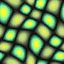
\includegraphics[height=0.25in]{../pixgen/data/scales.png}
    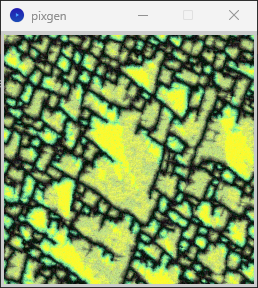
\includegraphics[height=1.0in]{images/pix_scales_7.png}
    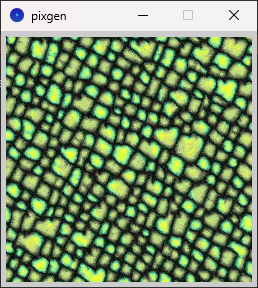
\includegraphics[height=1.0in]{images/pix_scales_11.png}
    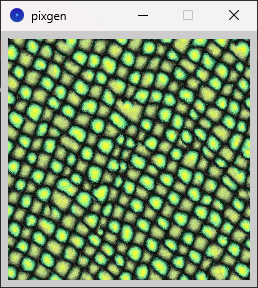
\includegraphics[height=1.0in]{images/pix_scales_15.png}
    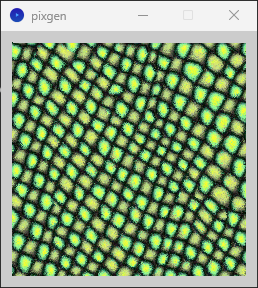
\includegraphics[height=1.0in]{images/pix_scales_23.png}
}
Pixel: multiple passes \\
\adjustbox{center}{
    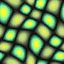
\includegraphics[height=0.25in]{../pixgen/data/scales.png}
    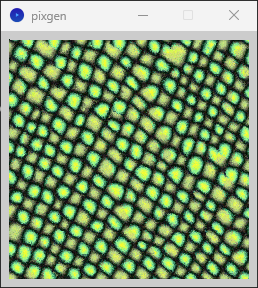
\includegraphics[height=1.0in]{images/pix_scales_onepass.png}
    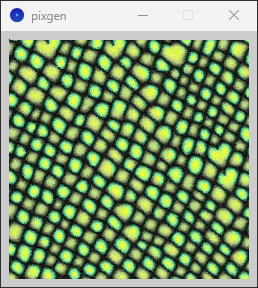
\includegraphics[height=1.0in]{images/pix_scales_twopass.png}
    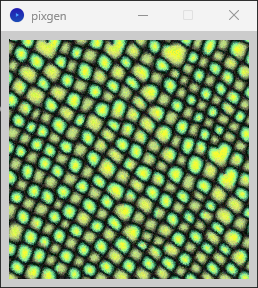
\includegraphics[height=1.0in]{images/pix_scales_threepass.png}
}
Pixels: sample search method \\
\adjustbox{center}{
    \includegraphics[height=0.25in]{../pixgen/data/text.png}
    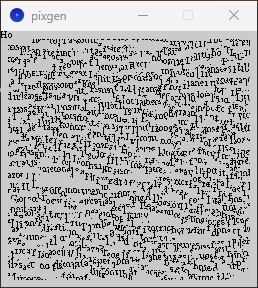
\includegraphics[height=1.0in]{images/pix_text_monte.png}
    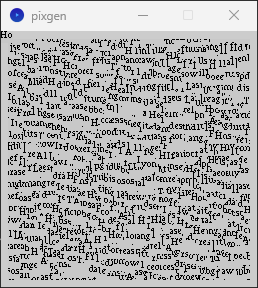
\includegraphics[height=1.0in]{images/pix_text_exhaustive.png}
}
Pixels: raster scan vs center growth \\
\adjustbox{center}{
    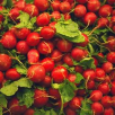
\includegraphics[height=0.25in]{../pixgen/data/tomatoe.png}
    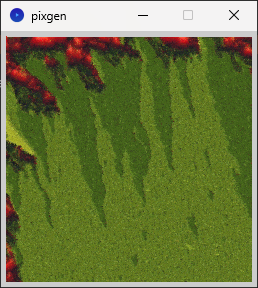
\includegraphics[height=1.0in]{images/tomatoe_garbage_small_window.png}
    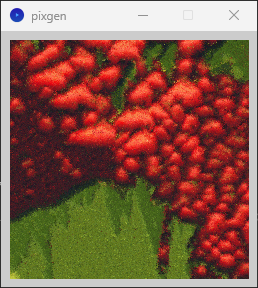
\includegraphics[height=1.0in]{images/tomatoe_center_small_window.png}
}
Patches: patch size \\
\adjustbox{center}{
    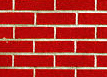
\includegraphics[height=0.25in]{../patchgen/data/brick.png}
    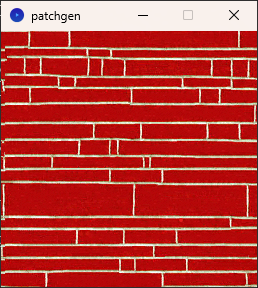
\includegraphics[height=1.0in]{images/patch_brick_8_4.png}
    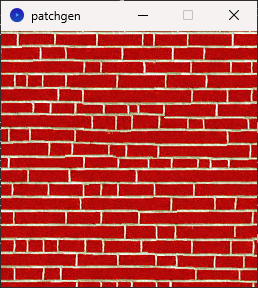
\includegraphics[height=1.0in]{images/patch_brick_16_8.png}
    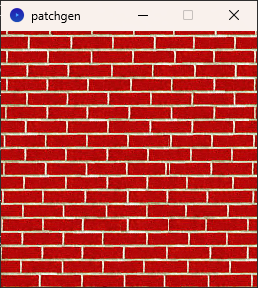
\includegraphics[height=1.0in]{images/patch_brick_32_24.png}
}
Patches: overlap size \\
\adjustbox{center}{
    \includegraphics[height=0.25in]{../patchgen/data/text.png}
    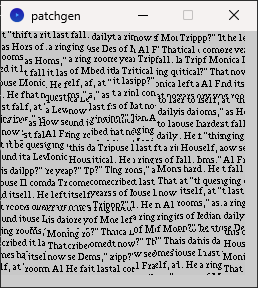
\includegraphics[height=1.0in]{images/patch_text_overlap_2.png}
    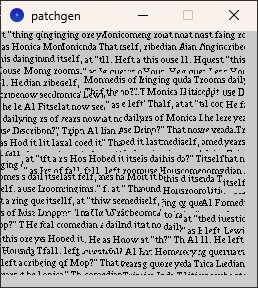
\includegraphics[height=1.0in]{images/patch_text_overlap_4.png}
    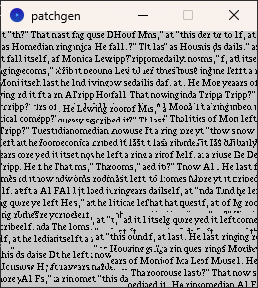
\includegraphics[height=1.0in]{images/patch_text_overlap_6.png}
    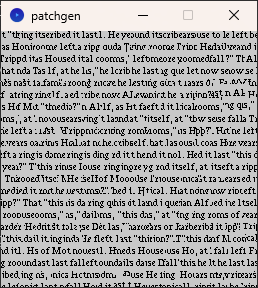
\includegraphics[height=1.0in]{images/patch_text_overlap_8.png}
    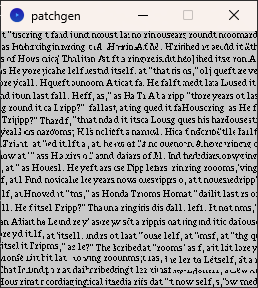
\includegraphics[height=1.0in]{images/patch_text_overlap_10.png}
}

Patches: some impressive results \\
\adjustbox{center}{
    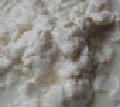
\includegraphics[height=0.25in]{../pixgen/data/cheese.png}
    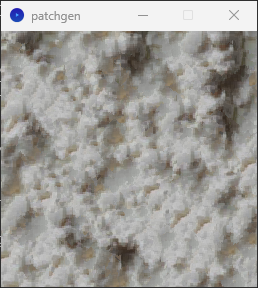
\includegraphics[height=1.0in]{images/patches_good_cheese.png}
    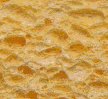
\includegraphics[height=0.25in]{../patchgen/data/bread.png}
    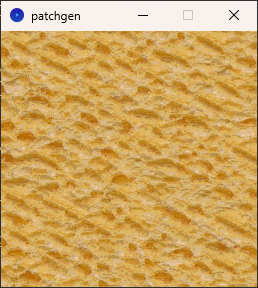
\includegraphics[height=1.0in]{images/patches_good_bread.png}
    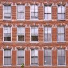
\includegraphics[height=0.25in]{../patchgen/data/building.png}
    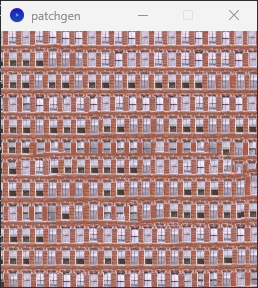
\includegraphics[height=1.0in]{images/patches_good_building.png}
}

\section{Analysis}
The pixel generation method is heavily influenced by window size both in output quality
and computation time. The first row of Results shows how the output changes as
the correlation window size increases from 5, 7, 11, 15, 23 from left to right.
At smaller sizes, execution is extremely fast but the generation often gets
stuck in areas of largely repeated garbage. As the window size increases, we
also see a lot more stable macro-scale patterns maintained from the original.

Interestingly, the pixel method seems to greatly benefit from multiple passes
over the same image. In Results, we demonstrate the difference between a single,
double, and triple pass over the same generated image. Later passes seem to
smooth out sharp discontinuities and seems while making interior color gradients
and transitions more gradual.

Next we compare the results of performing random Monte Carlo sampling of the
example image with an exhaustive search of all pixels for a good match. In
textures such as the text, the method benefits greatly from the exhaustive
search as the single-pixel level sparse binary detail is hard to coherently
maintain even with a relatively high number of random samples. In the generated
image, 1000 samples are taken for each pixel which although results in a
text-like appearance, doest not use true letters as found in the example. Line
structure is still lacking as I had to use a relatively small window size to
enable the brute force search through the exemplar.

Finally for the pixel method, we can see the difference between initializing a
single pixel in the top left and iterating in raster scan order vs initializing a
small patch in the center and growing outwards. In general through my
experimentation, I found that the raster scan method seemed to get stuck in
repeating regions more often than center growth. This could be due to fixed
``shape'' of the valid pixels in the correlation kernel. The variety in
surrounding pixels from the center growth method seems to slightly hedge against
runaway regions of color. That being said, this example seems quite poor for
both methods.

As the paper pointed out, the patch quilting method is heavily effected by the
size of the patches sampled from the example image. We can see the results for a
brick texture at patch sizes 8, 16, and 32. Although the lines are maintained in
the small examples, the macro-scale pattern of the brick is lost. Ideally we
want the patch to be large enough to encapsulate both the horizontal and
vertical brick divisions for any given window placement.

The overlap size generally doesn't effect most image generation as long as it is
set generally wide enough to capture patterns. In some extremely structured
images such as the text, this extreme diminishing returns can be seen. The
larger the overlap region, the better the random samples can be evaluated based
on their fit to the current generated region. A tiny overlap does not provide
the necessary information to characterize compatibility of larger scale
patterns, such as the rigid line structure as found in the text image. In
general an overlap of 1/4 to 1/2 of the patch size is optimal.

Finally, I demonstrate a few more textures that I feel the patch-based quilting
method performed very well at generating. For textures that have repeating medium to large
scale patterns, the patch method seems to vastly out perform the purely pixel
based method. The pixel method on the other hand seems to generate excellent
textures that contain lots of high frequency detail, and small to medium size
elements (such as the scales texture). The pixel method introduces high
frequency color noise to its generated images while the patches purely use
source material, only potentially introducing artifacts at the patch edges. 

\section{Code}
\subsection{Pixelgen}
\begin{lstlisting}
import java.util.Arrays;

PImage exampleImg;
color[] outputArr;
int outWidth, outHeight;

float ErrorThreshold = 30.0;
int MonteCarloSamples = 300;

color[] candidateMatches;
int kernelSize = 23;
float sigma = float(kernelSize) / 6.4; 
float[] gaussianWeights = generateGaussianKernel(kernelSize, sigma);
boolean[] dummyValidMask;

final color INVALID_COLOR = color(0, 0);


int IX(int x, int y) { return y * outWidth + x; }

class Pair {
  int x;
  int y;
  Pair(int x, int y) {
    this.x = x;
    this.y = y;
  }
}

class ScoredColor {
  color col;
  float score;
  
  ScoredColor(color col, float score) {
    this.col = col;
    this.score = score;
  }
}


void initOutputArr(int w, int h) {
  outputArr = new color[w * h];
  outWidth = w;
  outHeight = h;
  Arrays.fill(outputArr, INVALID_COLOR);
}

int winWidth = 256, winHeight = 256;

void settings() {
  size(winWidth, winHeight);
}

void setup() {
  exampleImg = loadImage("cheese.png");
  exampleImg.loadPixels();
  initOutputArr(winWidth, winHeight);
  candidateMatches = new color[exampleImg.pixels.length];
  noLoop();
  randomSeed(1337);
}

float computeSimilarity(int exX, int exY, float[] weights, boolean[] validMask, int outX, int outY) {
  int k = kernelSize / 2;
  //int validCount = 0;
  float accumScore = 0.0;
  float weightSum = 0.0;
  for(int i = 0; i < kernelSize; i++) {
    for(int j = 0; j < kernelSize; j++) {
      int oy = outY + (i - k);
      int ox = outX + (j - k);
      color cmp = outputArr[oy * outWidth + ox];
      if(cmp == INVALID_COLOR) continue;
      
      int y = exY + (i - k);
      int x = exX + (j - k);
      color sample = exampleImg.pixels[y * exampleImg.width + x];
      
      float d = colorDistance(sample, cmp);
      float w = weights[i * kernelSize + j];
      //float v = (validMask[i * kernelSize + j]) ? 1.0 : 0.0;
      //float v = (cmp == INVALID_COLOR) ? 0.0 : 1.0;

      float result = d * w;
      //float result = d;
      
      accumScore += result;
      weightSum += w;
    }
  }
  return (weightSum > 0.0) ? (accumScore / weightSum) : 0.0; // Normalize
  //return accumScore; // Normalize
}

color findClosestMatch(int outX, int outY) {
  int k = kernelSize / 2;
  Arrays.fill(candidateMatches, INVALID_COLOR);
  int matches = 0;
  float lowestScore = 10000000.0;
  color closestColor = INVALID_COLOR;
  for(int y = k; y < exampleImg.height - k; y++) {
    for(int x = k; x < exampleImg.width - k; x++) {
      float score = computeSimilarity(x, y, gaussianWeights, dummyValidMask, outX, outY);
      //if(score < ErrorThreshold) {
      //  scoredColors[matches] = new ScoredColor(exampleImg.pixels[y * exampleImg.width + x], score);
      //  matches++;
      //}
      score += random(ErrorThreshold); //randomly jitter score to introduce variance
      if(score < lowestScore) {
        lowestScore = score;
        closestColor = exampleImg.pixels[y * exampleImg.width + x];
      }
    }
  }
  //if(matches == 0) println("NO MATCHES", lowestScore);
  
  //color randPick = candidateMatches[floor(random(matches))];
  //return randPick;
  return closestColor;
}

color findClosestMatchMonte(int outX, int outY, int numTries) {
  int k = kernelSize / 2;
  float lowestScore = 100000000.0;
  color closest = color(1.0, 0.0, 1.0);
  for(int i = 0; i < numTries; i++) {
    int exY = floor(random(k, exampleImg.height - k));
    int exX = floor(random(k, exampleImg.width - k));
    color sample = exampleImg.pixels[exY * exampleImg.width + exX];
    float score = computeSimilarity(exX, exY, gaussianWeights, dummyValidMask, outX, outY);
    if(score < lowestScore) {
      lowestScore = score;
      closest = sample;
    }
  }

  return closest;
}

void initializeTextureSingleCornerPixel(int k) {
  // sample a random pixel from original examplar and place it at the starting point in the output
  int ry = floor(random(exampleImg.height));
  int rx = floor(random(exampleImg.width));
  color randInitialColor = exampleImg.pixels[ry * exampleImg.width + rx];
  outputArr[IX(k, k)] = randInitialColor;
}

void iterateFillTopLeft(int k) {
    for(int y = k + 1; y < outWidth - k; y++) {
    for(int x = k; x < outWidth - k; x++) {
      color match = findClosestMatchMonte(x, y, MonteCarloSamples);
      //color match = findClosestMatch(x, y);
      outputArr[IX(x, y)] = match;
    }
    if(y % 10 == 0) {
        println(y);
    }
  }
}

void initializeTextureTopLeftPatch(int patchSize) {
  int p = patchSize;
  copyRegion(exampleImg.pixels, exampleImg.width, exampleImg.height, 
             floor(random(p, exampleImg.width - p)), floor(random(p, exampleImg.height - p)),
             p, p,
             outputArr, outWidth, outHeight, 0, 0);
}

void initializeTextureCenterPatch(int centerSize) {
  int c = centerSize;
  copyRegion(exampleImg.pixels, exampleImg.width, exampleImg.height, 
             floor(random(c, exampleImg.width - c)), floor(random(c, exampleImg.height - c)),
             centerSize, centerSize,
             outputArr, outWidth, outHeight, outWidth/2 - centerSize/2, outHeight/2 - centerSize/2);
}

void iterateFillGrowCenter(int centerSize) {
  int cx = outWidth / 2;
  int cy = outWidth / 2;
  int x = centerSize/2;
  int y = centerSize/2;
  int k = kernelSize/2;
  
  Pair blankPair = new Pair(0, 0);
  Pair[] pairs = new Pair[outWidth * 2 + outHeight * 2];
  int pairCount = 0;
  
  int xlim = cx - k - 1;
  int ylim = cy - k - 1;
  int cnt = 0;
  while(x < xlim && y < ylim) {
    // generate border cells to center grow
    for(int i = -x; i <= x; i++) {
      pairs[pairCount++] = new Pair(cx + i, cy + y);
      pairs[pairCount++] = new Pair(cx + i, cy - y);
    }
    
    for(int i = -y; i <= y; i++) {
      pairs[pairCount++] = new Pair(cx + x, cy + i);
      pairs[pairCount++] = new Pair(cx - x, cy + i);
    }
    if(x < xlim) x++;
    if(y < ylim) y++;
    
    shufflePairArray(pairs, pairCount);
    for(int j = 0; j < pairCount; j++) {
      Pair p = pairs[j];
      color match = findClosestMatchMonte(p.x, p.y, MonteCarloSamples);
      //color match = findClosestMatch(p.x, p.y);
      outputArr[IX(p.x, p.y)] = match;
    }
    //println("\n");
    //for(int i = 0; i < pairCount; i++)
    //  print (pairs[i].x, pairs[i].y, " ");
    
    Arrays.fill(pairs, 0, pairCount, blankPair);
    pairCount = 0;
    if((x + y) % 20 == 0) {
      println(x, y);
    }
  }
}

void generateTexture() {
  int k = kernelSize / 2;
  //initializeTextureSingleCornerPixel(k);
  initializeTextureTopLeftPatch(12);
  iterateFillTopLeft(k);
  //iterateFillTopLeft(k);
  //iterateFillTopLeft(k);
  
  //initializeTextureCenterPatch(12);
  //iterateFillGrowCenter(3);
}

void draw() {
  loadPixels();
  //image(exampleImg, 0, 0);
  //copyImage(exampleImg.pixels, 3, 3, outputArr, outWidth, outHeight, kernelSize/2, kernelSize/2);
  println("begin gen");
  generateTexture();
  println("end gen");
  arrayCopy(outputArr, pixels);
  updatePixels();
  Arrays.fill(outputArr, INVALID_COLOR);
}

float[] generateGaussianKernel(int ksize, float sigma) {
  int half = ksize / 2;
  float[] kernel = new float[ksize * ksize];
  float sum = 0;
  
  // Compute kernel values
  for (int y = -half; y <= half; y++) {
    for (int x = -half; x <= half; x++) {
      int index = (y + half) * ksize + (x + half);
      //if(x == 0 && y == 0) {kernel[index] = 0.0; continue;}
      kernel[index] = gaussian(x, y, sigma);
      sum += kernel[index];
    }
  }

  // Normalize
  for (int i = 0; i < kernel.length; i++) {
    kernel[i] /= sum;
  }

  return kernel;
}

// Gaussian function
float gaussian(float x, float y, float sigma) {
  float coeff = 1.0 / (TWO_PI * sigma * sigma);
  float exponent = -(x * x + y * y) / (2 * sigma * sigma);
  return coeff * exp(exponent);
}

float colorDistance(color c1, color c2) {
  float r1 = red(c1), g1 = green(c1), b1 = blue(c1);
  float r2 = red(c2), g2 = green(c2), b2 = blue(c2);
  
  return dist(r1, g1, b1, r2, g2, b2);  // Processing's dist() function
}

void copyRegion(color[] src, int srcW, int srcH, int srcX, int srcY, int copyW, int copyH, 
                color[] dest, int destW, int destH, int destX, int destY) {
  for (int y = 0; y < copyH; y++) {
    for (int x = 0; x < copyW; x++) {
      int srcXPos = srcX + x;
      int srcYPos = srcY + y;
      int destXPos = destX + x;
      int destYPos = destY + y;

      // Ensure we are within bounds of both images
      if (srcXPos >= 0 && srcXPos < srcW && srcYPos >= 0 && srcYPos < srcH &&
          destXPos >= 0 && destXPos < destW && destYPos >= 0 && destYPos < destH) {
        
        int srcIndex = srcYPos * srcW + srcXPos;
        int destIndex = destYPos * destW + destXPos;

        dest[destIndex] = src[srcIndex]; // Copy pixel
      }
    }
  }
}

void shufflePairArray(Pair[] array, int pairCount) {
  for (int i = pairCount - 1; i > 0; i--) {
    int j = int(random(i + 1)); // Pick a random index from 0 to i
    // Swap array[i] and array[j]
    Pair temp = array[i];
    array[i] = array[j];
    array[j] = temp;
  }
}
\end{lstlisting}
\subsection{Patchgen}
\begin{lstlisting}
import java.util.Arrays;

boolean shouldGen = true;
PImage exampleImg;
color[] outputArr;
int outWidth, outHeight;

int patchSize = 32;
int patchOverlap = 12;
color[] samplePatch = new color[patchSize * patchSize];
int numPatchSamples = 1024;

final color INVALID_COLOR = color(0, 0);
//final float MAX_COLOR_DIST = sqrt(255*255 * 3);
final float MAX_COLOR_DIST = 255*255 * 3;


void initOutputArr(int w, int h) {
  outputArr = new color[w * h];
  outWidth = w;
  outHeight = h;
  Arrays.fill(outputArr, INVALID_COLOR);
}

int winWidth = 256, winHeight = 256;
void settings() {
  size(winWidth, winHeight);
}

void setup() {
  exampleImg = loadImage("building.png");
  exampleImg.loadPixels();
  initOutputArr(winWidth, winHeight);
  randomSeed(1337);
  //noLoop();
}


void getRandomPatch(color[] patch) {
  Arrays.fill(patch, INVALID_COLOR);
  int rx = floor(random(exampleImg.width - patchSize));
  int ry = floor(random(exampleImg.height - patchSize));
  for(int i = 0; i < patchSize; i++) {
    for(int j = 0; j < patchSize; j++) {
      patch[i * patchSize + j] = exampleImg.pixels[(ry + i) * exampleImg.width + (rx + j)];
    }
  }
}

void initializeTextureTopLeft() {
  getRandomPatch(samplePatch);
  copyRegion(samplePatch, patchSize, patchSize, 0, 0, patchSize, patchSize,
             outputArr, outWidth, outHeight, 0, 0);
}

class CostMap {
  int h;
  int w;
  float[] map;
  float[] hmap;
  int[] cuts;
  int[] hcuts;
  
  CostMap(int h, int w) {
    this.w = w;
    this.h = h;
    this.map = new float[w * h];
    this.hmap = new float[w * h];
    this.cuts = new int[h]; // what column to cut at for each row
    this.hcuts = new int[h]; // what column to cut at for each row
    
    Arrays.fill(map, 0.0);
    Arrays.fill(hmap, 0.0);
  }
}

CostMap createCostMap(color[] patch, int outX, int outY) {
  CostMap costMap = new CostMap(patchSize, patchOverlap);
  if(outX > 0) {
    for(int y = 0; y < patchSize; y++) {
      for(int x = 0; x < patchOverlap; x++) {
        float cost = 0.0;
        int ix = (y + outY) * outWidth + (x + outX);
        if(ix < outputArr.length) 
          cost = colorDistance(patch[y * patchSize + x], outputArr[ix]);
        costMap.map[y * patchOverlap + x] = cost*cost;
      }
    }
  }
  return costMap;
}

CostMap createCostMapHoriz(color[] patch, int outX, int outY) {
  CostMap costMap = new CostMap(patchSize, patchOverlap);
  if(outY > 0) {
    for(int y = 0; y < patchOverlap; y++) {
      for(int x = 0; x < patchSize; x++) {
        float cost = 0.0;
        int ix = (y + outY) * outWidth + (x + outX);
        if(ix < outputArr.length) 
           cost = colorDistance(patch[y * patchSize + x], outputArr[ix]);
        costMap.map[x * patchOverlap + y] = cost*cost;
      }
    }
  }
  return costMap;
}

void drawCostMapVert(CostMap vcm, int outX, int outY) {
  for(int y = 0; y < vcm.h; y++) {
    for(int x = 0; x < vcm.w; x++) {
      float cost = vcm.map[y * vcm.w + x];
      float intensity = cost / MAX_COLOR_DIST;
      color col = color(intensity * 255.0);
      if (vcm.cuts[y] == x) {
        //col = color(255.0, 0.0, 0.0);
      } else {  
        //continue;
      }
      outputArr[(y + outY) * outWidth + (x + outX)] = col;
    }
  }
}

void drawCostMapHoriz(CostMap cm, int outX, int outY) {
  for(int y = 0; y < cm.w; y++) {
    for(int x = 0; x < cm.h; x++) {
      float cost = cm.map[x * cm.w + y];
      float intensity = cost / MAX_COLOR_DIST;
      color col = color(intensity * 255.0);
      if (cm.cuts[x] == y) {
        //col = color(255.0, 0.0, 0.0);
      } else {  
        //continue;
      }
      outputArr[(y + outY) * outWidth + (x + outX)] = col;
    }
  }
}

float getOverlapCost(CostMap cm) {
  float sum = 0;
  for(int i = 0; i < cm.map.length; i++) {
    sum += cm.map[i];
  }
  return sum;
}


float minCutCostMap(CostMap cm) {
  // Create a 2D array to store minimum costs
  float[][] minCost = new float[cm.h][cm.w];
  // Create a 2D array to store the column used to reach each cell
  int[][] prevCol = new int[cm.h][cm.w];
  
  // Initialize the first row with costs from the map
  for (int x = 0; x < cm.w; x++) {
    minCost[0][x] = cm.map[x];
    prevCol[0][x] = x; // Starting column
  }
  
  // Process each row from the second one to the bottom
  for (int y = 1; y < cm.h; y++) {
    for (int x = 0; x < cm.w; x++) {
      // Get current cell's cost
      float cellCost = cm.map[y * cm.w + x];
      
      // Initialize with a large value
      minCost[y][x] = Float.MAX_VALUE;
      
      // Check the three possible previous cells (left diagonal, above, right diagonal)
      int search = 1;
      for (int dx = -search; dx <= search; dx++) {
        int prevX = x + dx;
        
        // Skip if previous column is out of bounds
        if (prevX < 0 || prevX >= cm.w) continue;
        
        // Calculate total cost through this path
        float pathCost = minCost[y-1][prevX] + cellCost;
        
        // If this path is cheaper, update the minimum cost and previous column
        if (pathCost < minCost[y][x]) {
          minCost[y][x] = pathCost;
          prevCol[y][x] = prevX;
        }
      }
    }
  }
  
  // Find the column with minimum cost in the last row
  float minBottomCost = Float.MAX_VALUE;
  int minBottomCol = 0;
  
  for (int x = 0; x < cm.w; x++) {
    if (minCost[cm.h-1][x] < minBottomCost) {
      minBottomCost = minCost[cm.h-1][x];
      minBottomCol = x;
    }
  }
  
  // Backtrack to find the optimal path
  cm.cuts[cm.h-1] = minBottomCol; // Set the bottom row's cut
  
  for (int y = cm.h-1; y > 0; y--) {
    // The previous column is determined by the prevCol array
    cm.cuts[y-1] = prevCol[y][cm.cuts[y]];
  }
  return minBottomCost;
}

void drawPatch(color[] patch, CostMap vcm, CostMap hcm, int outX, int outY) {
  for(int py = 0; py < patchSize; py++) {
    for(int px = vcm.cuts[py]; px < patchSize; px++) {
      if(py < hcm.cuts[px]) continue;
      int ix = (py + outY) * outWidth + (px + outX);
      if(ix >= outputArr.length || (px + outX) >= outWidth) continue;
      outputArr[(py + outY) * outWidth + (px + outX)] = patch[py * patchSize + px];
    }
  }
}

void generateTexture() {
  //initializeTextureTopLeft();
  float lowestCost = Float.MAX_VALUE;
  color[] bestPatch = new color[samplePatch.length];
  CostMap bestVCM = new CostMap(patchSize, patchOverlap);
  CostMap bestHCM = new CostMap(patchSize, patchOverlap);
        
  int patchStep = patchSize - patchOverlap;
  int numTilesX = floor(outWidth / (patchStep));
  int numTilesY = floor(outHeight / (patchStep));
  //int numTilesX = 6;
  //int numTilesY = 6;
  
  for(int ty = 0; ty < numTilesY; ty++) {
    for(int tx = 0; tx < numTilesX; tx++) {
      lowestCost = Float.MAX_VALUE;
      for(int i = 0; i < numPatchSamples; i++) {
        getRandomPatch(samplePatch);
        CostMap costMap = createCostMap(samplePatch, tx*patchStep, ty*patchStep);
        CostMap costMapHoriz = createCostMapHoriz(samplePatch, tx*patchStep, ty*patchStep);
        float overlapCost = getOverlapCost(costMap);
        overlapCost += getOverlapCost(costMapHoriz);
        if(overlapCost < lowestCost) {
          arrayCopy(samplePatch, bestPatch);
          lowestCost = overlapCost;
          arrayCopy(costMap.map, bestVCM.map);
          arrayCopy(costMapHoriz.map, bestHCM.map);
        }
      }
      
      minCutCostMap(bestVCM);
      minCutCostMap(bestHCM);
      
      drawPatch(bestPatch, bestVCM, bestHCM, tx*patchStep, ty*patchStep);
      //drawCostMapVert(bestVCM, tx*patchStep, ty*patchStep);
      //drawCostMapHoriz(bestHCM, tx*patchStep, ty*patchStep);
    }
  }
}

void draw() {
  if(!shouldGen) {
    delay(500);
    return;
  }
  
  loadPixels();
  generateTexture();
  arrayCopy(outputArr, pixels);
  updatePixels();
  shouldGen = false;
}

void copyRegion(color[] src, int srcW, int srcH, int srcX, int srcY, int copyW, int copyH, 
                color[] dest, int destW, int destH, int destX, int destY) {
  for (int y = 0; y < copyH; y++) {
    for (int x = 0; x < copyW; x++) {
      int srcXPos = srcX + x;
      int srcYPos = srcY + y;
      int destXPos = destX + x;
      int destYPos = destY + y;

      // Ensure we are within bounds of both images
      if (srcXPos >= 0 && srcXPos < srcW && srcYPos >= 0 && srcYPos < srcH &&
          destXPos >= 0 && destXPos < destW && destYPos >= 0 && destYPos < destH) {
        
        int srcIndex = srcYPos * srcW + srcXPos;
        int destIndex = destYPos * destW + destXPos;

        dest[destIndex] = src[srcIndex]; // Copy pixel
      }
    }
  }
}

float colorDistance(color c1, color c2) {
  float r1 = red(c1), g1 = green(c1), b1 = blue(c1);
  float r2 = red(c2), g2 = green(c2), b2 = blue(c2);
  
  return dist(r1, g1, b1, r2, g2, b2);  // Processing's dist() function
}

void keyPressed() {
   shouldGen = true;
}
\end{lstlisting}
\end{document}